% $Id: INF_Poster.tex 7714 2011-08-31 17:34:46Z tkren $
%
% TU Wien - Faculty of Informatics
% poster template
%
% This template is using the beamer document class and beamerposter package, see
% <http://www.ctan.org/tex-archive/macros/latex/contrib/beamer/>
% <http://www.ctan.org/tex-archive/macros/latex/contrib/beamerposter/>
% <http://www-i6.informatik.rwth-aachen.de/~dreuw/latexbeamerposter.php>
%
% For questions and comments send an email to
% Thomas Krennwallner <tkren@kr.tuwien.ac.at>
%

\documentclass[final,hyperref={pdfpagelabels=true}]{beamer}

\usepackage{TUINFPST}
\usepackage{minted}
\usepackage[export]{adjustbox}
\usepackage{lipsum}
\usepackage{longtable,booktabs}
\usetikzlibrary{matrix}
\usepackage{setspace}

% block styling
\setbeamercolor{block body}{fg=black,bg=white}
\setbeamercolor{block title}{fg=TuWienBlue,bg=white}
\setbeamertemplate{block begin}{
  \begin{beamercolorbox}{block title}%
    
\begin{tikzpicture}%
      \node[draw,rectangle,line width=3pt,rounded corners=0pt,inner sep=0pt]{%
        \begin{minipage}[c][2cm]{\linewidth}
          \centering\textbf{\insertblocktitle}
        \end{minipage}
      };
    \end{tikzpicture}%
  \end{beamercolorbox}
  \vspace*{1cm}
  \begin{beamercolorbox}{block body}%
}
\setbeamertemplate{block end}{
  \end{beamercolorbox}
  \vspace{2cm}
}

% figure numbers
% https://tex.stackexchange.com/questions/127145/beamer-presentation-figure-has-no-number
\setbeamertemplate{caption}[numbered]

\title[Computational Logic] {
    DRAT Proofs without Harmful \\ Reason Clause Deletions \\
    \&\\
    Complete and Fast \\ DRAT Proof Checking
}
\author[aclopte@gmail.com]{\texorpdfstring
	{Johannes Altmanninger, \today}
	{Johannes Altmanninger}}
\institute[]{%
  Technische Universit{\"a}t Wien\\[0.25\baselineskip]
  Institute of Logic and Computation\\[0.25\baselineskip]
  Arbeitsbereich: Formal Methods in Systems Engineering\\[0.25\baselineskip]
  Betreuer: Associate Prof. Dipl.-Ing. D.Phil. Georg Weissenbacher
}
\titlegraphic{\adjincludegraphics[height=52mm,trim={0 0 {.37\width} 0},clip]{forsyte.png}}
\date[\today]{\today}
\subject{epilog}
\keywords{SAT solving, proof systems, implementation}

%%%%%%%%%%%%%%%%%%%%%%%%%%%%%%%%%%%%%%%%%%%%%%%%%%%%%%%%%%%%%%%%%%%%%%%%%%%%%%%%%%%%%%
% Display a grid to help align images 
% \beamertemplategridbackground[1cm]

% for crop marks, uncomment the following line
% \usepackage[cross,width=88truecm,height=123truecm,center]{crop}

%%%%%%%%%%%%%%%%%%%%%%%%%%%%%%%%%%%%%%%%%%%%%%%%%%%%%%%%%%%%%%%%%%%%%%%%%%%%%%%%%%%%%%

\begin{document}

\begin{frame}[fragile]
  \begin{columns}[t]
    \begin{column}{.45\textwidth}

    \begin{block}{Motivation}
        \begin{itemize}
            \item SAT solvers produce DRAT proofs that are incorrect$^\texttt{a}$
             due to spurious deletions
            of \textbf{reason clauses}
            \item proof checkers remedy this by ignoring reason deletions
            \item handling reason deletions requires a complex algorithm
            with possible performance impact
        \end{itemize}
    \end{block}

    \begin{block}{Problem}
        \begin{itemize}
                \item unsatisfiable propositional formula
        	$ F =
        	(x \lor y) \land
            	(x \lor \overline{y}) \land
            	(\overline{x} \lor y) \land
            	(\overline{x} \lor \overline{y})
        	$
        	% \vspace{1cm}

		\item redundant clauses (according to criteria RUP or RAT) \\
			can be added without affecting satisfiability of
			the formula
		\item proof of unsatisfiability adds and deletes clause
		until deriving the empty (unsatisfiable) clause $\square$

		\begin{tabular}{lll}
        		\texttt{1: add} & $x$			& \hspace{1cm} addition of redundant clause		\\
        		\texttt{2: del} & $x \lor y$		& \hspace{1cm} deletion of subsumed clause (always fine)		\\
        		\textcolor{red}{\texttt{3: del}} & \textcolor{red}{$x$}			& \hspace{1cm} \textcolor{red}{deletion of reason clause (loss of information)}		\\
        		\texttt{4: add} & $\square$		& \hspace{1cm} addition of redundant conflict clause	\\
		\end{tabular}
        \end{itemize}

	\vspace{1cm}

	\begin{columns}[T]
    	    \begin{column}{.35\textwidth}
        	    \begin{itemize}
			\item clause $x$ is the \textbf{reason} for $y$
			and $\overline{y}$
            	    	\item deleting $x$ makes the proof incorrect
			\item many SAT solvers produce such proofs $\rightarrow$
			proof checkers ignore reason deletions
        	    \end{itemize}
    	    \end{column}
    	    \begin{column}{.6\textwidth}
                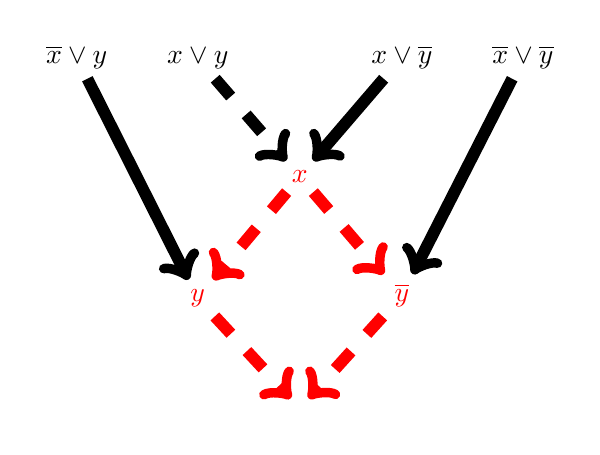
\begin{tikzpicture}[
                        dep/.style={->,line width=1.5mm},
                        del/.style={dep,dash pattern=on 3mm off 3mm},
                        bad/.style={red}
                    ]
                  \matrix (m) [matrix of math nodes,row sep=3em,column sep=1.5em,minimum width=1.5em]
                  {
                      \overline{x}\lor{}y	& x\lor{}y	&	  		& x\lor{}\overline{y} & \overline{x}\lor{}\overline{y}	\\
                     			&	& \textcolor{red}{x}	&		& 				\\
                     			& \textcolor{red}{y}	&	  		& \textcolor{red}{\overline{y}}  &   				\\
                     			&	& \textcolor{red}{\square}		&		&				\\
                  };
                  \draw [del]     (m-1-2) -- (m-2-3);
                  \draw [dep]     (m-1-4) -- (m-2-3);

                  \draw [dep]     (m-1-1) -- (m-3-2);
                  \draw [del,bad] (m-2-3) -- (m-3-2);

                  \draw [dep]     (m-1-5) -- (m-3-4);
                  \draw [del,bad] (m-2-3) -- (m-3-4);

                  \draw [del,bad] (m-3-4) -- (m-4-3);
                  \draw [del,bad] (m-3-2) -- (m-4-3);

                  % \draw [dep] (m-1-1) -- (m-2-2);
                  % \draw [dep,dash pattern=on 3mm off 3mm,red] (m-1-2) -- (m-2-2);
                  % \draw [dep] (m-1-3) -- (m-2-2);
                \end{tikzpicture}
    	    \end{column}
	\end{columns}

    \end{block}

    \begin{block}{Contributions}
        \begin{itemize}
		\item provide patches for SAT solvers to produce correct proofs
		\item extension of SICK incorrectness certificate, giving
		a counter-example for an incorrect proof
		\item implement efficient checker to measure performance
		impact of reason deletions
        \end{itemize}
    \end{block}


    \begin{block}{Avoiding Reason Deletions in Solvers}
	\begin{itemize}
	    \item \texttt{DRUPMiniSat}-based solvers delete reason clauses
	    but do not undo corresponding assignments
            \item remedy: emit a unit clause before deleting a reason clause
            --- yields correct proofs that match the solver's behavior
	    \item we implemented this in \texttt{DRUPMiniSat}\\
		patch shown below --- reason clauses are called \texttt{locked}
            \item similar patch for the 2018 SAT competition winner
	\end{itemize}
	\vspace{0.5cm}
        {\footnotesize
            \begin{minted}[]{diff}
@@ -632,9 +632,13 @@ void Solver::removeSatisfied(vec<CRef>& cs)
         Clause& c = ca[cs[i]];
+        if (output != NULL && locked(c)) {
+            Lit unit = c[0];
+            fprintf(output, "%i 0\n",
+                    (var(unit) + 1) * (-2 * sign(unit) + 1));
+        }
         removeClause(cs[i]);
            \end{minted}
        }
    \end{block}
    \end{column}

    \begin{column}{.45\textwidth}
    \begin{block}{SICK Format}
        \begin{itemize}
            \item \emph{small} artifact to \emph{efficiently} certify
            incorrectness of a proof
            \item can be verified with our tool \texttt{sick-check}
        \end{itemize}
        \vspace{.5cm}
        incorrect DRAT proof for $F$:

	\begin{tabular}{lll}
    		\texttt{1: del} & $x \lor y$		& \\
    		\texttt{2: add} & $x$			& \\
    		\texttt{3: add} & $\square$		& \\
	\end{tabular}

        \vspace{.5cm}
	SICK certificate disproving RAT of clause $x$:
        \begin{align*}
            \texttt{proof\_format}	&= \texttt{DRAT-arbitrary-pivot}		\\
	    \texttt{proof\_step}	&= 2 \text{\quad (Failed line in the proof)}	\\
	    \texttt{natural\_model}	&= \{\overline{x}, \overline{y}\}		\\
	    \texttt{failing\_clause}	&= \overline{x} \lor y				\\
	    \texttt{failing\_model}	&= \{\}						\\
	    \texttt{pivot}		&= x						
        \end{align*}
    \end{block}
    \begin{block}{Checker Implementation: \texttt{rate}}
        \begin{itemize}
            \item efficiently handles reason deletions
            \item competitive performance (Figure \ref{fig:cactus-time})
            \item available at \url{https://github.com/krobelus/rate}
            \item written in Rust
        \end{itemize}
    \begin{figure}
        \centering
        \caption{Distribution of Proof Checkers' runtime\label{fig:cactus-time}}
        \includegraphics[scale=2]{../p/cactus-time.png}
    \end{figure}

    \textbf{Insight:} an excessive number of reason
    deletions may effect longer checking runtime (Figure
    \ref{fig:correlation-reason-deletions-time-delta}).  Find more details
    at \url{https://github.com/krobelus/rate-experiments}.

    \vspace{.5cm}

    \begin{figure}
        \centering
        \caption{Overhead in seconds of handling reason deletions\label{fig:correlation-reason-deletions-time-delta}}
        \includegraphics[scale=2]{../p/correlation-reason-deletions-time-delta.png}
    \end{figure}

    \begin{singlespace}
        \footnotesize
        $^\texttt{a}$ For simplicity and brevity, this poster assumes
        correctness of a DRAT proof to be defined in terms of specified DRAT
        as per \emph{A. Rebola-Pardo and A. Biere, ``Two Flavors of DRAT'',
        Pragmatics of SAT, vol. 2018.}
    \end{singlespace}

    \end{block}
    \end{column}
  \end{columns}
\end{frame}

\end{document}

%%% Local Variables:
%%% TeX-PDF-mode: t
%%% TeX-debug-bad-boxes: t
%%% TeX-master: t
%%% TeX-parse-self: t
%%% TeX-auto-save: t
%%% reftex-plug-into-AUCTeX: t
%%% End:
